\documentclass[sigconf,nonacm,prologue,table]{acmart}
\usepackage{listings}

%% labels
%% sections:    "sec"
%% definitions: "def"
%% equations:   "eq"
%% figures:     "fig"
%% tables:      "tab"

%% packages
\usepackage{amsmath}
\usepackage{pgfplots}
\usepackage{subcaption}
\usepackage{commath}
\usepackage[utf8]{inputenc}
\usetikzlibrary{positioning, arrows.meta, shapes, calc}
\usepackage{titlesec}
%% \usepackage{tikz}

\pagenumbering{arabic}

%% hide ACM reference
\settopmatter{printacmref=false}

%% hide copyright
\renewcommand\footnotetextcopyrightpermission[1]{}

%% \pagestyle{plain}
\settopmatter{printfolios=true}

\numberwithin{equation}{section}

\theoremstyle{definition}
\newtheorem{definition}{Definition}

\theoremstyle{remark}
\newtheorem*{remark}{Remark}

\captionsetup[subfigure]{
    labelfont=bf,
    textfont=normalfont,
}
\renewcommand{\thesubfigure}{\Roman{subfigure}}

\definecolor{rowA}{gray}{0.9}
\definecolor{rowB}{gray}{0.8}

\newcommand{\rplus}{\mathbb{R}_{\geq 0}}
\newcommand{\rpos}{\mathbb{R}_{>0}}

\begin{document}
\title{Doppler Multicurve}
\subtitle{April 2025}
\date{April 2025}

\author{Austin Adams}
\affiliation{}
\email{austin@whetstone.cc}

\author{Matt Czernik}
\affiliation{}
\email{matt@whetstone.cc}

\author{Rohan Kulkarni}
\affiliation{}
\email{rohan@zora.co}

\author{Cooper Kunz}
\affiliation{}
\email{cooper@whetstone.cc}

\begin{teaserfigure}
\caption*{
    \hspace{\textwidth}
    }
\end{teaserfigure}

\renewcommand{\shortauthors}{Adams et all}

\begin{abstract}
Financial markets are increasingly becoming internet native. One-size-fits-all token launchpads and liquidity bootstrapping protocols have failed to meet the needs of token creators and their communities. Developers increasingly want onchain markets with application-specific customizations. We introduce \textsc{Doppler Multicurve}, a new primitive for onchain issuance that enables multiple price curves to be specified during an initial auction or liquidity bootstrapping phase, which can then be tailored to a specific use case or application's needs. In doing so, developers have the expressivity necessary to reduce maximal extractable value (MEV), and enable more capital-efficient liquidity formation.
\end{abstract}

\maketitle

\section{Introduction} \label{sec:introduction}
When utilizing a concentrated liquidity automated market maker (CLAMM), static bonding curve-based projects place one constant liquidity position for buyers. However, one constant liquidity placement comes with a subtle but impactful downside: significantly more tokens are available for trading at the cheapest prices on the position, leading to an outsized portion of the token supply sold to the earliest buyers (who are generally MEV bots). MEV bots, in turn, quickly dump these cheap shares when new buyers enter the market, extracting value from both the new buyers and the token project. Additionally, the wider the position across the price spectrum, the more outsized this price dilation effect is, and potential downside for users.

\begin{figure}[H]
    \centering
        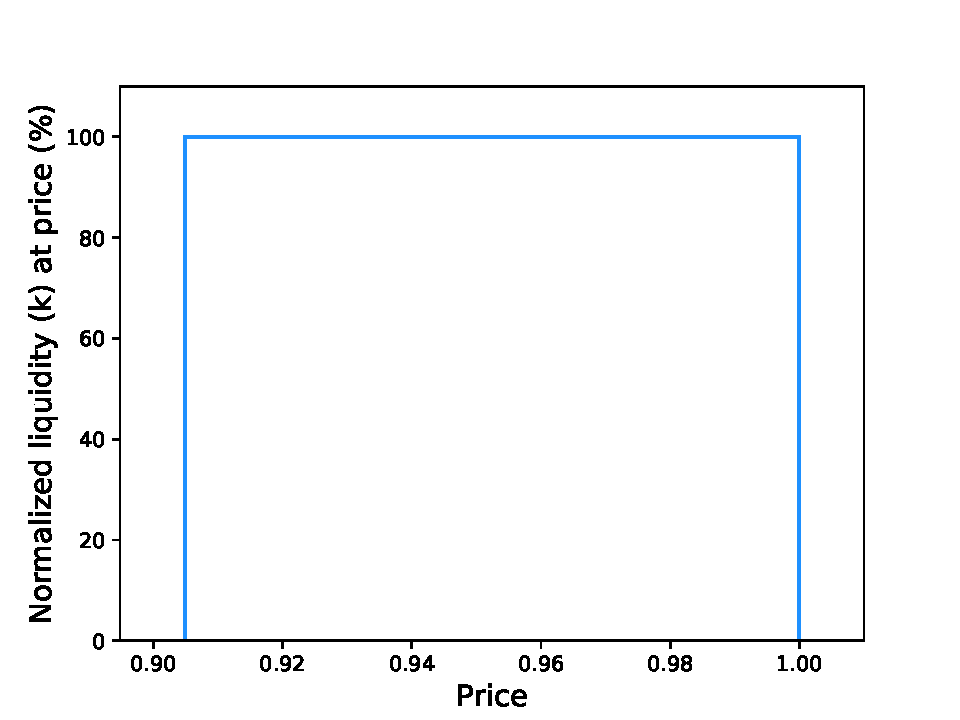
\includegraphics[scale=0.425]{images/1.pdf} \caption{A Single Constant Liquidity Position}
\end{figure}

\textsc{Doppler Multicurve} turns this on its head and addresses one of the biggest limitations of liquidity-bootstrapping protocol’s integration with CLAMMs. Instead of placing one constant liquidity position (shown in Figure 1), integrators specify their desired curves, which in itself is entirely managed by \textsc{Multicurve}. \textsc{Multicurve} is entirely compatible with the current \textsc{Doppler Protocol} \cite{Adams25} ecosystem.

In practice, this means that \textsc{Multicurve} creates a curve mimicking a log-normal curve utilizing individual concentrated liquidity positions, which aims to sell a constant number of tokens in each price bucket. An example of this is shown above in Figure 1. Additionally, while not shown in the above figure, multiple of these curves can be placed, allowing customization of complex curves and price paths, entirely maintained and executed inside the existing Doppler position manager. Similar to all other Doppler features, it’s natively compatible with existing popular AMM integrations, such as \textsc{Uniswap}. 

Compared to a static bonding curve, \textsc{Multicurve} reduces sniping, leads to higher liquidity and prices, allows for a more customizable market structure, and lowers the cost of price discovery.


\section{Background} 
\label{sec:Background} 

Over the last year, there has been a significant increase in the number of bonding curve-based liquidity bootstrapping protocols such as pumpdotfun, clanker, and Meteora. This proliferation has resulted in a awide variety of different implementations with various market structure impacts. The bonding curve design utilized by most (with notable exceptions like pumpdotfun) utilizes an $x\cdot y=k$ concentrated-liquidity AMM (CLAMM), such as \textsc{Uniswap v3} \cite{Adams21}, as the matching engine for their protocols.

However, as previously stated, $x\cdot y=k$ AMMs have a major drawback for new token liquidity bootstrapping, where the amount of tokens sold by the protocol decreases as the price of the token goes up, which is guaranteed if there is any trading activity. By selling the most amount of tokens at the cheapest possible price, token projects that use these static bonding curves will have increased losses from sniping, increased cost of price discovery, and will result in overall lower user welfare. Additionally, we will show mathematically in the appendix that selling more tokens during the earlier trading period phase is a fundamental property of $x\cdot y=k$ AMMs, which is addressed through a layering technique pioneered by \textsc{Doppler Multicurve}.

\section{Single Curve} 
\label{sec:single}

At its core, \textsc{Doppler Multicurve} is first a collection of individual single log-normal curves. With multiple curves, integrators can describe increasingly complex curvatures by combining multiple single curves.

First, we describe the parameterization of a single curve. We note for brevity that we only describe the case where the new token is $token_0$.

To parameterize a single curve, integrators provide a $tickLower$, $tickUpper$, total token amount ($amount$) for bootstrapping liquidity, and desired steepness (known as $numPositions$). The $numPositions$ is the number of positions created by \textsc{Multicurve}.

$tickLower$ and $tickUpper$ refer to the placement of possible liquidity positions in CLAMMs and must satisfy the conditions enforced by the specific AMM.

To start, the total token amount, $amount$ is divided equally among all positions.

\begin{equation}
    positionTokens_i = \frac{amount}{numPositions}
\end{equation}

Next, in the $token_0$ case, each position ends at $tickUpper$ with the $tickLower$ of the the position linearly spanning from $tickLower$ to $tickUpper$. This is flipped accordingly in the $token_1$ case.

\begin{equation}
    tickLower_i = tickLower +  \lfloor \frac{i \cdot (tickUpper - tickLower)}{numPositions} \rfloor
\end{equation}

Due to both integer math and implementation details, each $tickLower_i$ is binned according to the $tickSpacing$. Depending on the configuration of the curve and the $numPositions$, this could result in multiple positions overlapping with the same $tickLower$ and $tickUpper$. This should be avoided due to unnecessary gas costs, but is accounted for in the implementation. 

Each position is placed from its calculated $tickLower_i$ to $tickUpper$. Each of these positions are given equal numbers of tokens with their $liquidity$ calculated at run time, resulting in a staircase-like liquidity structure, where positions closer to $tickUpper$ have more liquidity. This results in more tokens concentrated around that value than a constant liquidity position.

\begin{figure}[H]
    \centering
    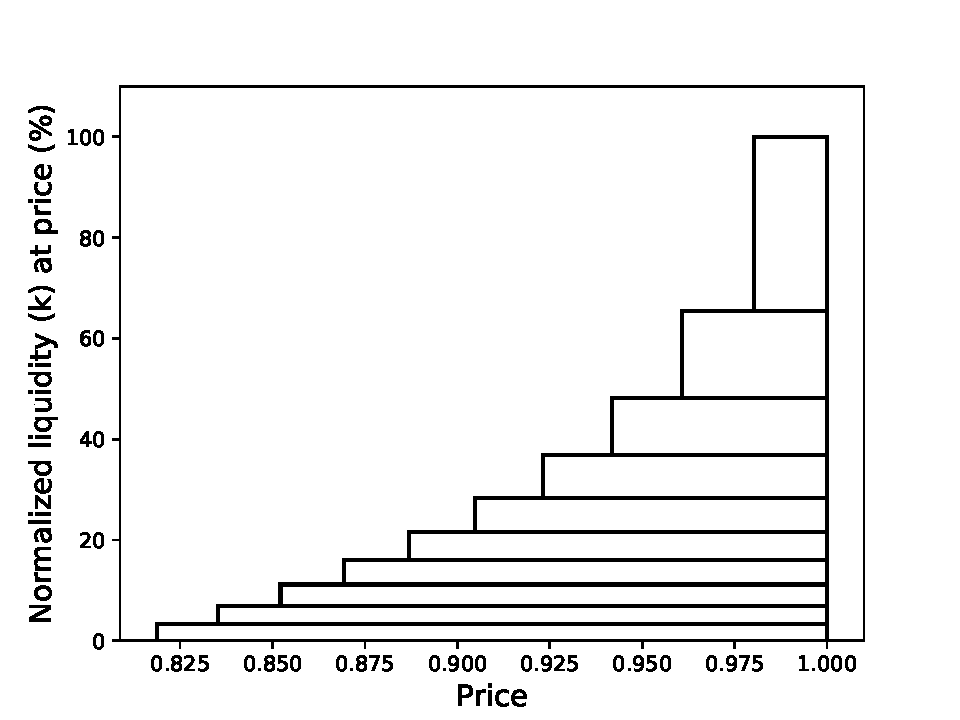
\includegraphics[scale=0.45]{images/10.pdf} 
     \caption{A selected single curve}
     \label{fig:fig2}
\end{figure}

In Figure 2, we show a sample implementation of the single curve design with $tickLower=-2000$ , $tickUpper=0$, $numPositions=10$\footnote{As $liquidity$ is normalized in the chart, $amount$ is arbitrary}. With more positions, the $liquidity$ of the system is more concentrated around global $tickUpper$ of the curve. More liquidity in the upper parts of the curve results in faster price accumulation and a higher average price execution. 

From these four parameters, every position in the curve can always be cheaply calculated ensuring that all positions are always tracked while additionally lowering the gas cost by maintaining less information inside onchain storage.

\section{Multicurve} 
\label{sec:multi}

In principle, \textsc{Multicurve} is a direct extension of a single curve, allowing integrators to provide multiple curve parameterizations that are then jointly managed by the \textsc{Doppler} position manager. By allowing integrators to place multiple curves, increasingly complex curvatures can be described, resulting in the ability to place bonding curves that are molded around the design of the token and the expected price path. As different token types will have different expected price paths, features, and timelines, the structure of the liquidity bootstrapping should also adapt to these features as well.

\begin{figure}[H]
    \centering
    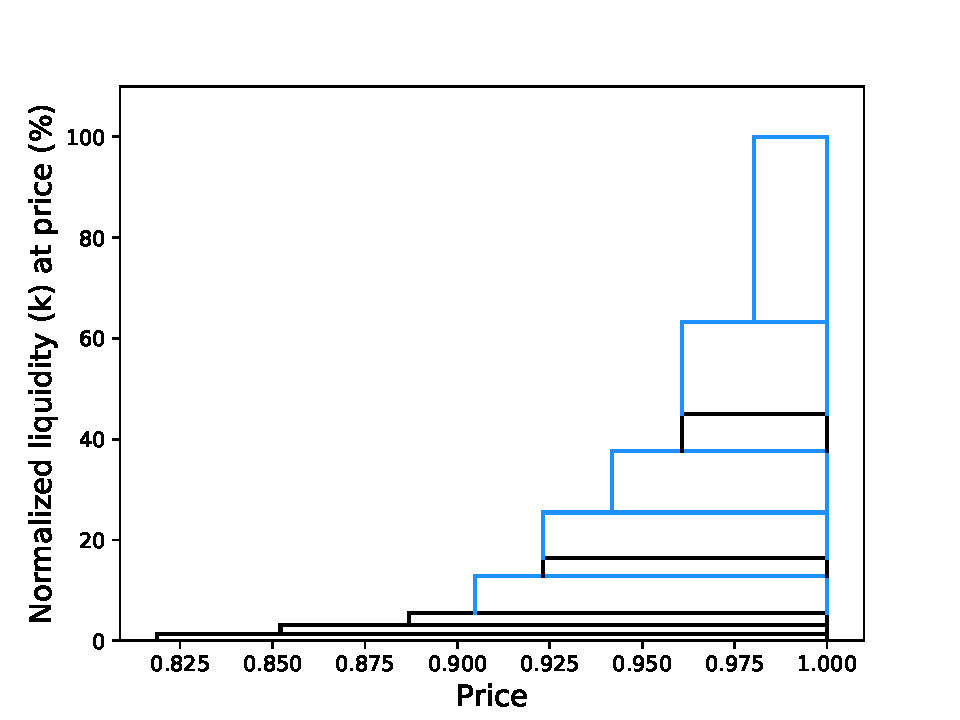
\includegraphics[scale=0.45]{images/5_10.pdf}
     \caption{Two selected multiple curvitures}
\end{figure}

An example \textsc{Multicurve} liquidity path is shown above. The two curves are $Curve_1$ colored in black with ($tickLower_1=-2000$ , $tickUpper_1=0$, $numPositions_1=5$, $tokenAmt_1=10\%$) and $Curve_2$ colored in blue with ($tickLower_2=-1000$ , $tickUpper_1=0$, $numPositions_1=5$, $tokenAmt_1=25\%$). This curve is designed to facilitate early price discovery from $Curve_1$ with thin but continuous liquidity. From there, a $Curve_2$ is layered over the first to lower price impact at higher prices. Both of these curves are entirely managed by the \textsc{Doppler} position manager

As an added feature, \textsc{Doppler} itself calculates the amount of the numeraire token (generally ETH, but there is no requirement) that will result in exiting the entire curve. This allows integrators to easily know how many tokens will be generated during initial liquidity bootstrapping. This also allows \textsc{Doppler} itself to calculate the optimal amount of the quote token (the token being sold) needed to bond. Finally, this ensures that \textsc{Doppler} has enough of the bootstrapping token liquidity to bond against as a safety check.

\section{Conclusion} 
\label{sec:users}

As more of the financial economy moves onchain, and internet capital markets become increasingly relevant, it is important to have practical mechanisms that can support their ambitions. The design of \textsc{Doppler Multicurve} is intended to simplify the integrator experience while allowing them to customize their capital markets to their application or implementation needs. Integrators pick what their starting and ending price of the token is, and then go end to end with cheaper price discovery. 

For one example, by utilizing just one single curve in \textsc{Multicurve}, Zora lowered the starting price of their tokens by 60x (from \$1,320 to \$22) with the same cost from sniping as a constant liquidity curve. 

By lowering the cost of sniping with high price precision, the tokens created on the protocol will result in higher prices and more liquidity, as less value will be extracted via sniping bots. By incorporating a second curve and iterating on the design according to market feedback, the cost of initial liquidity provision should continue to lower. 



\newpage

\appendix
\section{Mathematical Appendix} 
\label{sec:math}

To explain why a constant liquidity position leads to more tokens sold at cheaper prices, we first must explain what constant liquidity in concentrated liquidity math refers to. 

A good mental model is that $liquidity$ is the $k$ in the ever popular $x\cdot y=k$ equation.\footnote{We note that in the \textsc{Uniswap v3} model, liquidity is actually sqrt(k) due to implementation details, but this does not notably impact the directionality of the meaning.}  

First, we define the price $p$ as the reserves of $x$ divided by the reserves of $y$.

\begin{equation}
   p = \frac{x}{y}
\end{equation}

Next, we can rewrite and substitute $x$ to find the impact of $price$ increasing.

\begin{equation}
   k = y^2p
\end{equation}

Finally, we can rewrite to isolate $y$. 

\begin{equation}
  y = \sqrt{\frac{k}{p}}
\end{equation}

Since $p = \frac{x}{y}$, an increase in $price$ means that $y$ is more valuable than it previously was worth. We see that as the price increases, the amount of $y$ in the pool likewise must decrease. This is fairly obvious because users are buying $y$ with $x$ if the price is going up, resulting in more $x$ and less $y$ in the pool.

\begin{tikzpicture}
\begin{axis}[
    xlabel={Price},
    ylabel={$y = \sqrt{k/p}$},
    xmin=0, xmax=10,
    ymin=0, ymax=5,
    domain=0.25:10,
    samples=100,
    title={Plot of $y = \sqrt{k/p}$ with $k = 10$},
]

% The main curve with k=4
\addplot[thick, black] {sqrt(10/x)};

% Add a legend
\legend{$k = 10$};
\end{axis}
\end{tikzpicture}

However, what is important to note is actually the shape of this graph. It is non-linear, meaning that the amount of tokens sold between two bins is not constant.

Now, we want to show that there always exists more tokens in earlier price bins than in later price bins if $k$ is constant in the bin. This results in the amount of $y$ sold to be larger at the earliest stages inside the liquidity pool. This effect results in an outsized portion of the token supply sold to the earliest buyers. 

To move between arbitrary prices in concentrated liquidity, we must buy all the tokens $y$ from $p$ to $p+\delta$.

To show that the amount $y$ is strictly decreasing from $p_1$ to $p_2$ if $p_2 > p_1$, we must show that the derivative of $y$ with respect to $price$ is always negative.

\begin{equation}
   \frac{dy}{dp}  = -\frac{\sqrt k}{2 p^{3/2}}
\end{equation}

This derivative is negative for all positive values of $p$ and $k$, which means the function is always decreasing as price increases. This results in more tokens sold at the earliest bins than later ones.

\begin{tikzpicture}
\begin{axis}[
    xlabel={Price},
    ylabel={$\frac{dy}{dp} = -\frac{\sqrt{k}}{2 \cdot price^{3/2}}$},
    xmin=0.1, xmax=10,
    ymin=-5, ymax=0,
    domain=0.5:10,
    samples=100,
    title={Derivative of $y = \sqrt{k/p}$ with respect to $p$},
]

% The main derivative curve with k=10
\addplot[thick, black] {-sqrt(10)/(2*x^(3/2))};

% Add a legend
\legend{$k = 10$};

% Add a horizontal asymptote at y=0
\draw[gray, dashed] (axis cs:0.1,0) -- (axis cs:10,0);

\end{axis}
\end{tikzpicture}

Additionally, the derivative is non-linear and increases rapidly around the earliest possible prices, resulting in this effect to be larger at the start of the price curve and for smaller token prices (which is what is commonly used for new token projects)

Overall, the main way to combat this effect is to utilize a shifting $k$ value, which is all implemented via \textsc{Doppler Multicurve}. As shifting the amount of $k$ between bins negates this non-linear decrease in the amount sold per bin.

\newpage

\bibliographystyle{ACM-Reference-Format}
\bibliography{main}

\section{Disclaimers}

\textbf{No Legal, Financial, or Investment Advice.} This document does not constitute legal advice, financial advice, investment advice, trading advice, or a recommendation of any kind by Doppler, its affiliates, or any of their respective officers, directors, managers, employees, agents, advisors, or consultants. No information contained herein should be relied upon as the basis for any investment decision, contract, or any other decision regarding engagement with Doppler or any of its projects.

\textbf{Forward-Looking Statements.} This document may contain forward-looking statements based on assumptions and beliefs of Doppler, its officers, or its affiliates. These statements are subject to known and unknown risks, uncertainties, and other factors, many of which are outside Doppler's control, that may cause actual outcomes to differ materially from the projections or expectations set forth in such statements. Doppler makes no obligation to update or revise any forward-looking statements to reflect subsequent events, developments, or changes in circumstances after the date on which such statements were made, except as required by law.

\end{document}
\endinput